\documentclass[tikz]{standalone}
\usepackage{amsmath}
\begin{document}
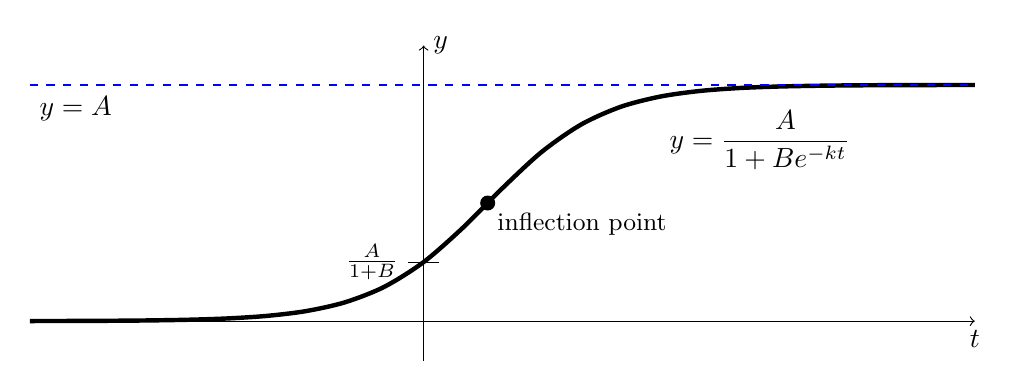
\begin{tikzpicture}[scale=1.0]

%\draw[black,fill=white] (-6,-1) rectangle (8,4);
%\draw[very thin,color=lightgray,step=0.5] (-3.4,-4.9) grid (3.4,0.9);
%\draw[very thin,color=gray,step=2] (-3.5,-5) grid (3.5,1);

\draw[->] (-5,0) -- (7.0,0) node[below] {$t$};
\draw[->] (0,-0.5) -- (0,3.5) node[right] {$y$};
       
\node[right] at (-5, 2.7){$y = A$};
\node[right] at (3, 2.3){$y = \dfrac{A}{1+Be^{-kt}}$};
\draw (0.2,0.75) -- (-0.2,0.75) node[left] {$\frac{A}{1+B}$};

\draw[domain=-5.0:7.0,smooth,variable=\x,black,ultra thick] plot ({\x},{3/(1 + 3/exp(1.35*\x))});
\draw[thick,blue,dashed] (-5,3) -- (7,3);

\draw [black,fill=black] (0.814,1.5) circle (2.5pt) node[below right] {\small inflection point};
\end{tikzpicture}
\end{document}
